\section{Otimização da Colônia de Formigas}

Na busca por alimento, as formigas utilizam de feromônios para encontrar o melhor caminho.
Isso acontece da seguinte maneira: cada formiga deposita feromônio ao se deslocar. A partir
da avaliação da quantidade de feromônio depositada por formigas que já passaram pelo local,
formigas subsequentes tem mais probabilidade de se mover em rotas que tem mais feromônios. Ao
decorrer do tempo os feromônios vão evaporando, apagando rastros que não foram reforçados. 
Com isso, caminhos que são percorridos por mais formigas tem mais chance de serem 
percorridos por outras formigas do que aqueles que foram percorridos por menos formigas e 
caminhos que foram percorridos á pouco tempo tem mais chance de serem percorridos que caminhos
percorridos a muito tempo. A quantidade de feromônio depositado é mais intensa no trajeto de volta,
quando a comida foi encontrada. Outro fator que é levado em consideração é a qualidade da comida
encontrada, de maneira que mais feromônio é depositado quanto melhor for a fonte de alimento encontrada.
A medida que mais formigas exploram o local e encontram alimento, esse procedimento tende a otimizar o
trajeto entre a fonte de alimento e a colônia.

Apesar dessa heurística utilizada pelas formigas ser interessante para se resolver problemas combinatórios 
do tipo NP(i.e., com complexidade não polinomial), são necessários algumas adaptações na construção
de um algoritmo computacional.

A seguir é apresentado a meta-heurística do ACO(\textit{Ant Colony Optimization}) algoritmo,
juntamente com observações relacionadas as diferenças entre a heurística do ACO e o
comportamento natural das formigas descrito anteriormente.

\subsection{Meta-heurística do ACO}

\begin{figure}[ht]
  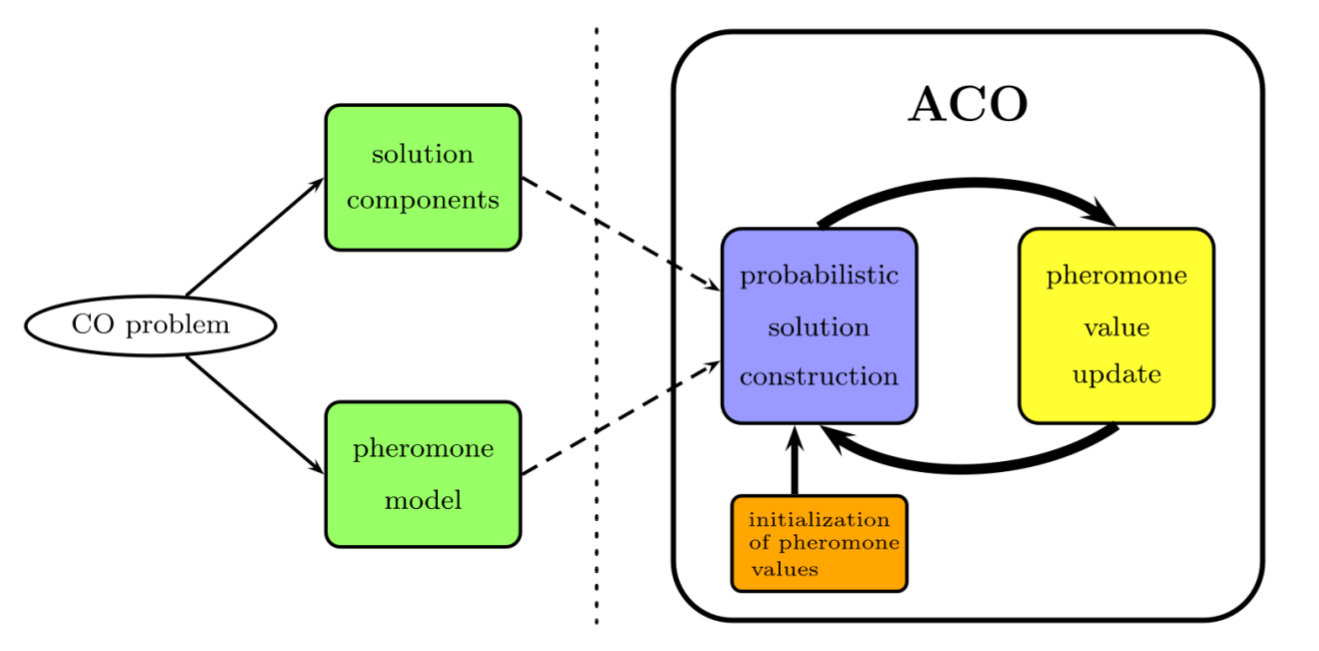
\includegraphics[width = 0.9 \linewidth]{imgs/meta_heuristica_aco}
  \label{diagrama_metaheuristica_aco}
  \caption{Diagrama de funcionamento da meta-heurística do ACO \cite{blum2005aco}}
\end{figure}

%Algoritmo
\begin{algorithm}[H]
  %Macros
  \SetKwBlock{AgendarAtividade}{AgendarAtividade}{fim}
  \SetKwBlock{Procedimento}{Procedimento}{fim}

  \Procedimento{
    \Enqto{$n < N_{MAX\_IT}$}{
      %\tcp*[f]{$N_{MAX\_IT}$ é o número máximo de iterações\\}
      \AgendarAtividade{
        ConstruirSolucoesFormigas\\
        AtualizarFeromonios\\
        %\tcp*[f]{opcional}\\
        \tcp{opcional:}
        AcoesGlobais
      }
    }
  }

  \caption{Pseudo código da meta-heurística do ACO\label{lst:meta-heuristica_aco}}
\end{algorithm}

A meta-heurística do ACO pode ser subdividida em três partes,
conforme proposto por \cite{doringo2004ant}: \textit{ConstruirSolucoesFormigas},
\textit{AtualizarFeromonios} e \textit{AcoesGlobais}.

\textit{ConstruirSolucoesFormigas} gerencia a movimentação de uma colônia de formigas
em torno dos nós vizinhos. A escolha do próximo nó é feita através de uma decisão
estocástica que é função da quantidade de feromônio no nós vizinhos e informação heurística.
Quando uma formiga encontra uma solução, ou enquanto a solução é construída, esta avalia a
qualidade da solução(completa ou parcial) que será utilizada pelo procedimento
\textit{AtualizarFeromonios} para decidir a quantidade de feromônio que será depositada.
Outro procedimento relevante na construção da solução é a eliminação de possíveis ciclos, utilizado
por exemplo, no problema do caixeiro viajante.

\textit{AtualizarFeromonios} é o processo que atualiza os traços de feromônio depositados pelas
formigas no espaço de busca. Os traços de feromônio podem aumentar, caso uma formiga tenha visitado
o nó/conexão em questão, ou diminuir, devido ao processo de evaporação do feromônio. Esse procedimento faz com 
que nós/conexões que foram visitados por muitas formigas ou por uma formiga e que tenha levado em
uma solução boa aumentem a probabilidade de serem visitados por futuras formigas. Semelhantemente, reduz 
a probabilidade de que nós que não foram visitados por novas formigas por muitas iterações sejam visitados
novamente. Logo, este procedimento evita a convergência a caminhos sub ótimos, favorecendo também a exploração
de novas regiões do espaço de busca.

Por fim, o procedimento \textit{AcoesGlobais} é utilizado para centralizar ações que não podem ser executadas
pelas formigas individualmente. Um exemplo de ações desse tipo é a filtragem de soluções ou o favorecimento de
regiões por meio de informações globais.

O procedimento \textit{AgendarAtividade} não necessariamente é uma instrução sequencial. Pode-se, portanto,
implementá-lo de maneira sequencial ou paralela, síncrona ou assincronamente. O tipo de abordagem que será
utilizada depende das características do problema que se deseja resolver.

\subsection{Exemplo de utilização}

\begin{figure}[ht]
  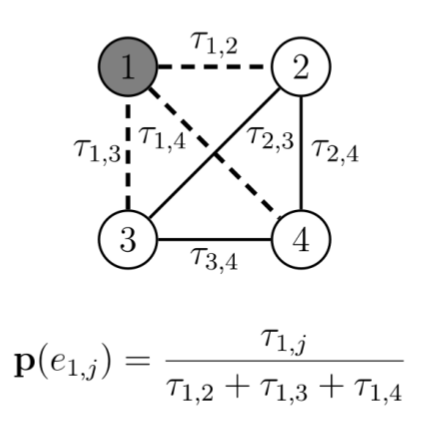
\includegraphics[width=0.32 \linewidth]{imgs/exemplo_aco_1}
  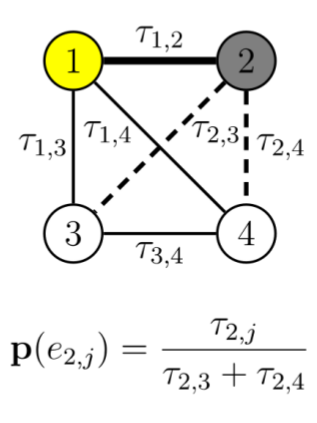
\includegraphics[width=0.32 \linewidth]{imgs/exemplo_aco_2}
  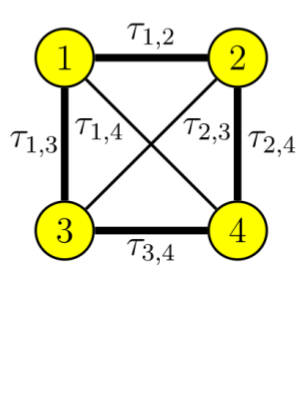
\includegraphics[width=0.32 \linewidth]{imgs/exemplo_aco_3}
  %\begin{subfigure}[b]
  %  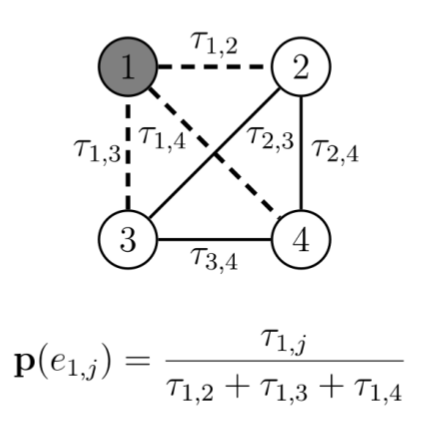
\includegraphics[width = 0.35 \linewidth]{imgs/exemplo_aco_1}
  %  \label{img:exemplo_aco_1}
  %\end{subfigure}
  %\begin{subfigure}
  %  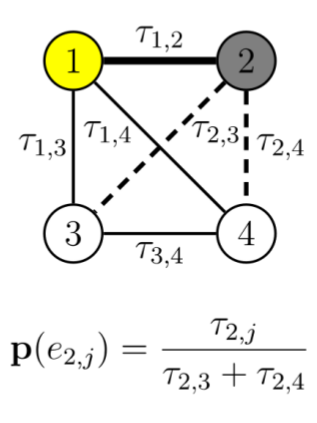
\includegraphics[width = 0.25 \linewidth]{imgs/exemplo_aco_2}
  %\end{subfigure}
  %\begin{subfigure}
  %  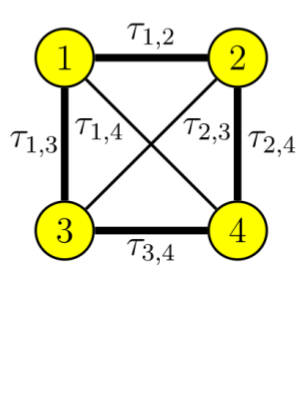
\includegraphics[width = 0.25 \linewidth]{imgs/exemplo_aco_3}
  %\end{subfigure}

  \label{img:exemp_aco}
  \caption{Example of the solution construction for a TSP problem}
  %It consists of 4 cities (modelled by a graph with 4 nodes; see Definition 1). The
  %solution construction starts by randomly choosing a start node for the ant;
  %in this case node 1. Figures (a) and (b) show the choices of the first,
  %respectively the second, construction step. Note that in both cases the
  %current node (i.e., location) of the ant is marked by dark gray color, and
  %the already visited nodes are marked by light gray color (respectively
  %yellow color, in the online version of this article). The choices of the ant
  %(i.e., the edges she may traverse) are marked by dashed lines. The probabilities
  %for the different choices (according to Eq. (4)) are given underneath the
  %graphics. Note that after the second construction step, in which we exemplary
  %assume the ant to have selected node 4, the ant can only move to node 3, and
  %then back to node 1 in order to close the tour. \cite{blum2005aco}}
\end{figure}

Definition 1. In the TSP is given a completely connected, undirected
graph $G = (V , E)$ with edge-weights. The nodes $V$ of this graph
represent the cities, and the edge weights represent the distances
between the cities. The goal is to find a closed path in $G$ that
contains each node exactly once (henceforth called a tour) and whose
length is minimal. Thus, the search space $S$ consists of all tours in
$G$. The objective function value $f(s)$ of a tour $s \in S$ is defined as
the sum of the edge-weights of the edges that are in $s$. The TSP can
be modelled in many different ways as a discrete optimization problem.
The most common model consists of a binary decision variable $X_e$ for
each edge in $G$. If in a solution $X_e = 1$, then edge e is part of the
tour that is defined by the solution. Concerning the AS approach, the
edges of the given TSP graph can be considered solution components,
i.e., for each $e_{i,j}$ is introduced a pheromone value $\tau_{i,j}$. The task of
each ant consists in the construction of a feasible TSP solution, i.e.,
a feasible tour. In other words, the notion of task of an ant changes
from “choosing a path from the nest to the food source” to “constructing
a feasible solution to the tackled optimization problem”. Note that with
this change of task, the notions of nest and food source loose their
meaning. Each ant constructs a solution as follows. First, one of the
nodes of the TSP graph is randomly chosen as start node. Then, the ant
builds a tour in the TSP graph by moving in each construction step from
its current node (i.e., the city in which she is located) to another
node which she has not visited yet. At each step the traversed edge is
added to the solution under construction. When no unvisited nodes are
left the ant closes the tour by moving from her current node to the
node in which she started the solution construction. This way of
constructing a solution implies that an ant has a memory $T$ to store
the already visited nodes. Each solution construction step is performed
as follows. Assuming the ant to be in node $v_i$ , the subsequent
construction step is done with probability:

\begin{equation}
  \emph{p}(e_{i,j}) = \frac{\tau_{i,j}}{\sum_{k \in \lbrace 1,...,
  \vert V \vert\rbrace, v_k \not\in T}\tau_{i,k}},
  \forall j \in \lbrace 1,...,\vert V \vert\rbrace, v_j \not\in T
\end{equation}

For an example of such a solution construction see Fig. \ref{img:exemp_aco}.
Once all ants of the colony have completed the construction of their solution,
pheromone evaporation is performed as follows:

\begin{equation}
  \tau_{i,j} \leftarrow (1-\rho)\cdot \tau_{i,j}, \forall \tau_{i,j}\in \mathcal{T}
\end{equation}

where $\mathcal{T }$ is the set of all pheromone values. Then the ants perform
their return trip. Hereby, an ant—having constructed a solution $s$— performs
for each $e_{i,j} \in s$ the following pheromone deposit:

\begin{equation}
  \tau_{i,j} \leftarrow \tau_{i,j} + \frac{Q}{f(s)}
\end{equation}

where $Q$ is again a positive constant and $f(s)$ is the objective function
value of the solution $s$. As explained in the previous section, the system
is iterated—applying $n_a$ ants per iteration—until a stopping condition
(e.g., a time limit) is satisfied.
Even though the AS algorithm has proved that the ants foraging behaviour
can be transferred into an algorithm for discrete optimization, it was 
generally found to be inferior to state-of-the-art algorithms. Therefore, 
over the years several extensions and improvements of the original AS
algorithm were introduced. They are all covered by the definition of the
ACO metaheuristic, which we will outline in the following section.

\subsection{Aplicação ao Problema}
